\documentclass[10pt,a4paper]{article}
\usepackage[utf8]{inputenc}
\usepackage[english]{babel}
\usepackage[T1]{fontenc}
\usepackage{amsmath}
\usepackage{amsfonts}
\usepackage{amssymb}
\usepackage{graphicx}
\usepackage{listings}
\author{Milan Tepic, Ivan Antunovic, Jung A Yoon, Peter von Zameck Glyscinski}
\title{Assignment 1}

\begin{document}
\maketitle

\section*{Task 1}
\subsection*{a)}
For Task Set 1 there is no feasible scheduling without having a task missing his deadline like we can see in figure \ref{fig:timming-diagram1}. 
\begin{figure}[h]
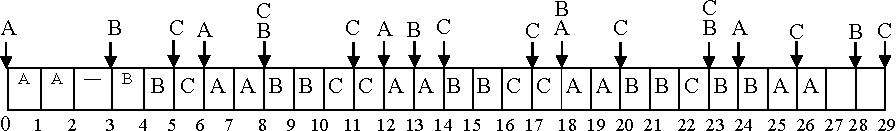
\includegraphics[width=\linewidth]{timing-diagram1.pdf}
\caption{Scheduling for Task Set 1}
\label{fig:timming-diagram1}
\end{figure}

For Task Set 2 there is a feasible scheduling which we can see in figure \ref{fig:timming-diagram2}.

\begin{figure}[h]
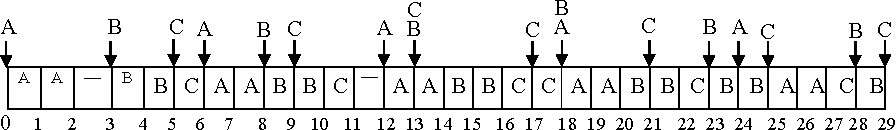
\includegraphics[width=\linewidth]{timing-diagram2.pdf}
\caption{Scheduling for Task Set 2}
\label{fig:timming-diagram2}
\end{figure}

\subsection*{b)}
If the task has the highest priority, schedulability is not possible, since the task $P_1$ will take all CPU time, without releasing CPU to handle other tasks.
\newline
If The task has not the highest priority, at least this task will miss its deadline because other tasks with a higher priority will delay it.
\subsection*{c)}
A could have the following values:
\begin{itemize}
\item[\textbf{15}] by having task $P_2$ be executed before line 2 of $P_1$ was executed.
\item[\textbf{21}] by having task $P_1$ be executed before line 2 of task $P_2$ was excecuted.
\item[\textbf{33}] by first executing the lines 1 and 2 of task $P_1$ then executing task $P_2$ and then executing line 3 of task $P_1$
\end{itemize}

\section*{Task 2}
\subsection*{a)}
\begin{itemize}
\item \textbf{No unbounded control statements at the beginning of a loop:}
\newline
Necessary because we need to know when it will be finished, or whether it will finish at all, in order to calculate WCET.

\item \textbf{No arbitrary recursive function calls:}
\newline
Necessary because we need to know the number of executions for the recurcive function calls in the design time in order to calculate WCET.

\item \textbf{No arbitrary dynamic data structure:}
In order to calculate WCET we need to know the executiontime of any operation on a dynamic data structure and therefore we need to know the length of the date structure in the design time.

\end{itemize}

\subsection*{b)}

\begin{figure}[h]
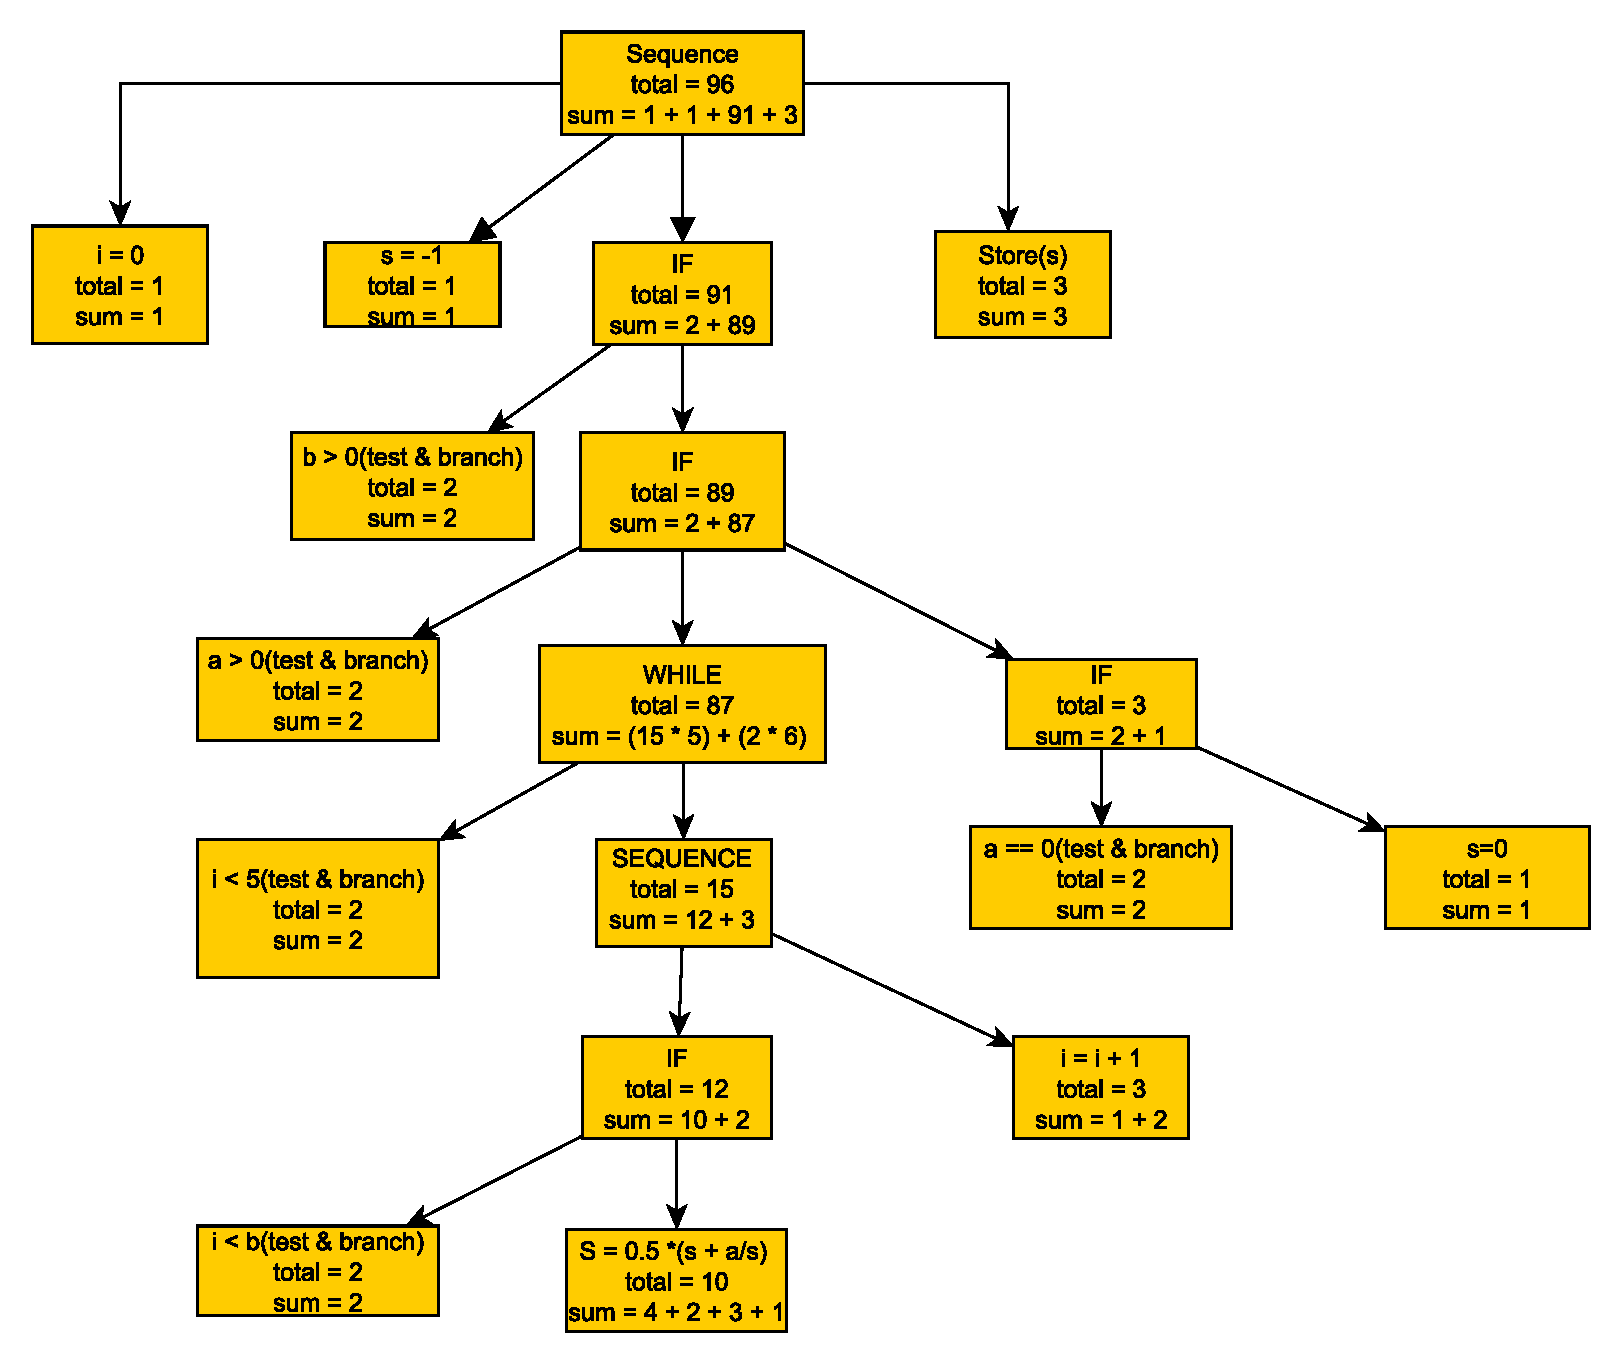
\includegraphics[width=\linewidth]{Ex1Task2b.pdf}
\end{figure}
\newpage
\section*{Task 3}

\subsection*{a)}
\begin{figure}[h]
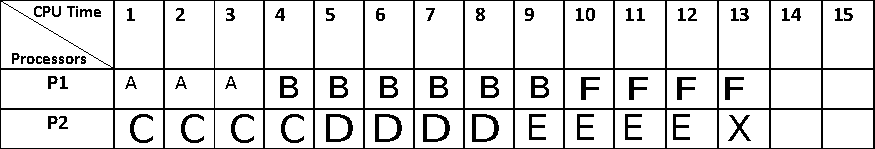
\includegraphics[width=\linewidth]{timing-diagram3a.pdf}
\end{figure}

\subsection*{b)}
\begin{figure}[h]
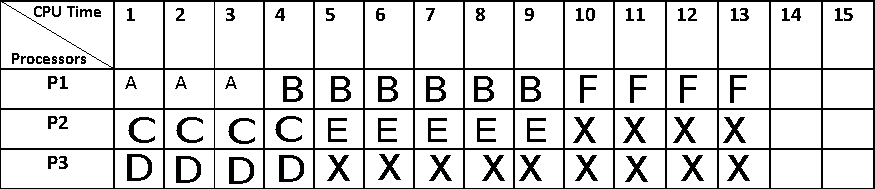
\includegraphics[width=\linewidth]{timing-diagram3b.pdf}
\end{figure}

\subsection*{c)}
\begin{figure}[h]
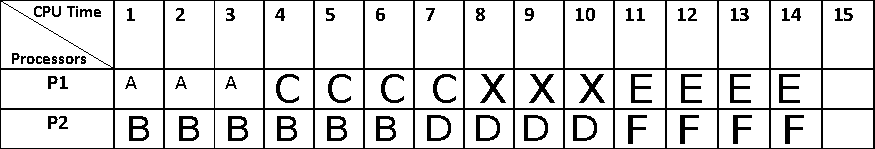
\includegraphics[width=\linewidth]{timing-diagram3c.pdf}
\end{figure}
\end{document}